
\chapter{相关研究综述}
\label{chap:relatedwork}
流行度预测问题自被提出以来,受到了学术界和产业界的广泛关注。本章从流行度的统计特征分析、流行度预测方法以及流行度预测问题的可预测性三个方面入手,对流行度预测领域的相关工作进行了系统的总结和归纳,以便读者更好地了解和掌握该领域的相关知识,进而更好地理解本文的工作。

\section{流行度的统计特征分析}
在线内容的流行度分析工作最早源于网站缓存策略的研究。Cunha等人\citep{cunha1995characteristics}在研究站点中网页的访问情况时发现,网页被访问频率的分布服从Zipf定律\citep{zipf2016human},也就是说:流行度排名为$i$的网页被用户访问的概率正比于$1/i$,如图\ref{fig:pageDist}所示。这一现象表明,网页的访问频次分布是不均匀的。Almeida等人\citep{almeida1996characterizing}在研究万维网中所有网页的访问频次时,也发现了同样的分布规律。
\begin{figure}[!htbp]
  \centering
  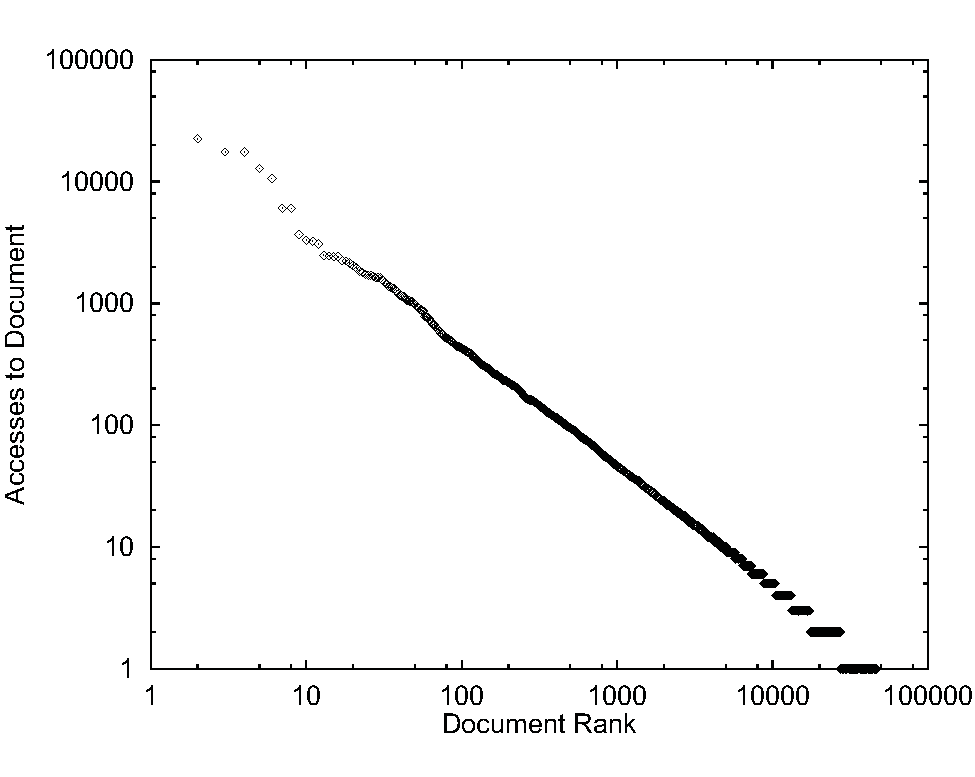
\includegraphics[width=0.75\textwidth]{docRank}
  \caption{站点中网页被访问的频率\citep{cunha1995characteristics}}
  \label{fig:pageDist}
\end{figure}

随着信息技术的发展,视频分享类网站和社交网络平台不断涌现,也引起了研究人员的关注。Gill等人\citep{gill2007youtube}收集并分析了视频网站Youtube\footnote{\url{https://www.youtube.com}}上视频的访问数据,发现视频的访问频次信息依然服从Zipf定律。Cha等人\citep{cha2009analyzing}对Youtube网站上的视频数据进行了详细的分析,发现网站中不同类别下的视频的观看数分布都服从幂律分布。Kwak等人\citep{kwak2010twitter}研究了社交网络平台Twitter\footnote{\url{https://twitter.com}}上消息的转发情况,发现参与消息转发的人数服从幂律分布,如图\ref{fig:tweetDist}所示。
\begin{figure}[!htbp]
  \centering
  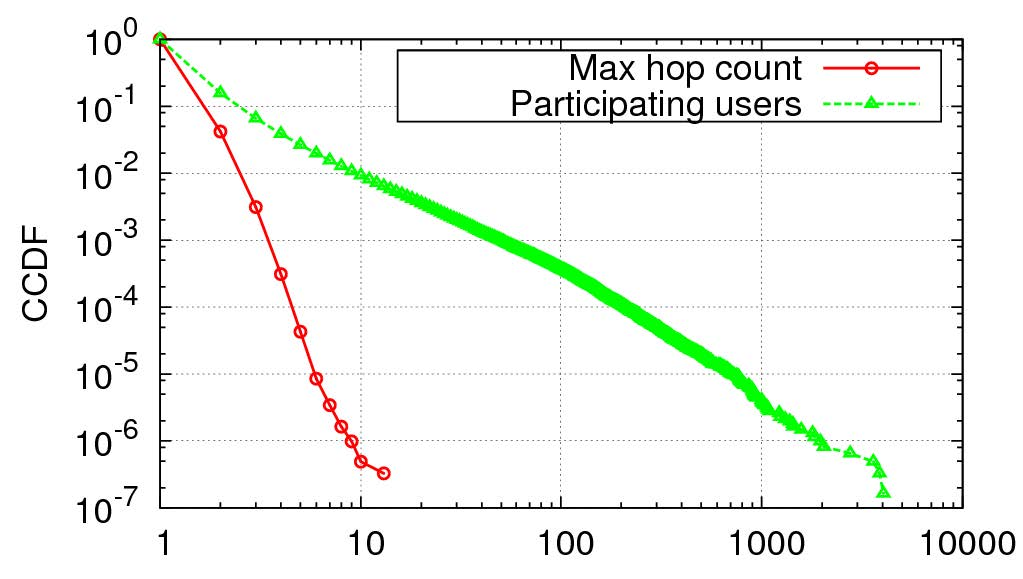
\includegraphics[width=0.75\textwidth]{tweetDist}
  \caption{Twitter平台中消息转发数和转发树深度的分布\citep{kwak2010twitter}}
  \label{fig:tweetDist}
\end{figure}

除了对宏观的流行度统计量的分析之外,还有一部分工作研究了流行度增长过程中的微观统计特征。Barabasi等人\citep{barabasi05}研究了人类的行为数据,发现人类的行为模式并不是服从传统方法中假设的泊松过程,而是存在爆发现象,并提出了一种基于事件优先级的排队模型来解释这一现象。爆发现象是指人类在参与某类事件时,大部分时间都处于沉寂状态,不会采取任何行为动作;中间夹杂了少数爆发区域,在爆发区域内会有大量的行为数据产生,如图\ref{fig:burst}所示。
\begin{figure}[!htbp]
  \centering
  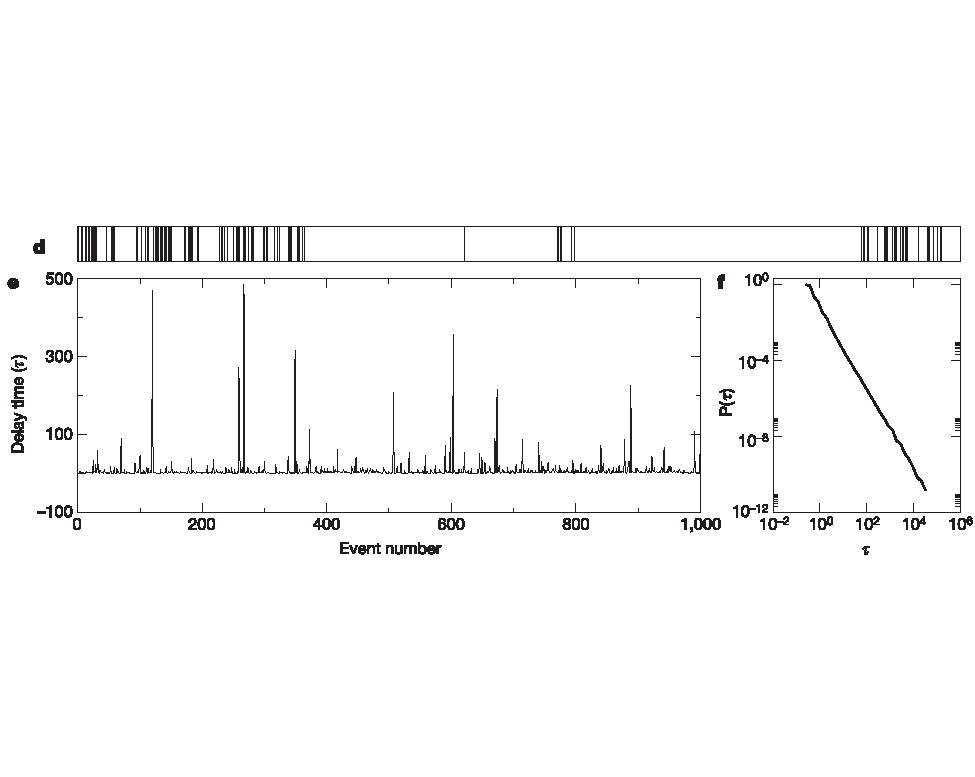
\includegraphics[width=1\textwidth]{burst}
  \caption{人类行为模式示例\citep{barabasi05}:(d)参与时间;(e)时间间隔;(f)时间间隔分布}
  \label{fig:burst}
\end{figure}

爆发现象在在线内容的流行度增长过程中十分常见。Kaltenbrunner等人\citep{kaltenbrunner2007description}研究了新闻评论网站Slashdot\footnote{\url{https://slashdot.org}}上新闻的评论情况,并对评论数据的时间间隔分布进行了分析。统计结果表明,评论数据的时间间隔分布是两个log-normal分布的混合,并且存在明显的周期现象。Bao等人\citep{bao2013cumulative}研究了新浪微博中消息的转发时间间隔数据,发现转发时间间隔分布服从幂律分布,这也说明了社交网络中消息的流行度累积过程中存在爆发现象。

除爆发现象外,研究人员还发现流行度的增长过程中存在着固定的模式。Yang等人\citep{yang2011patterns}研究了Twitter平台上消息的传播过程,提出了K-SC(K-Spectral Centroid)聚类方法,对消息的流行度变化过程进行聚类,将消息的流行度变化过程聚为六类,如图\ref{fig:pattern}所示。Crane等人\citep{crane2008robust}在研究Yotube网站中视频的观看数据时发现,视频的观看到达时间服从幂律分布,呈现出明显的``爆发-衰落"现象。此外,Costa等人\citep{ferraz2015rsc}还发现流行度增长过程中呈现出明显的周期性特点。
\begin{figure}[!htbp]
  \centering
  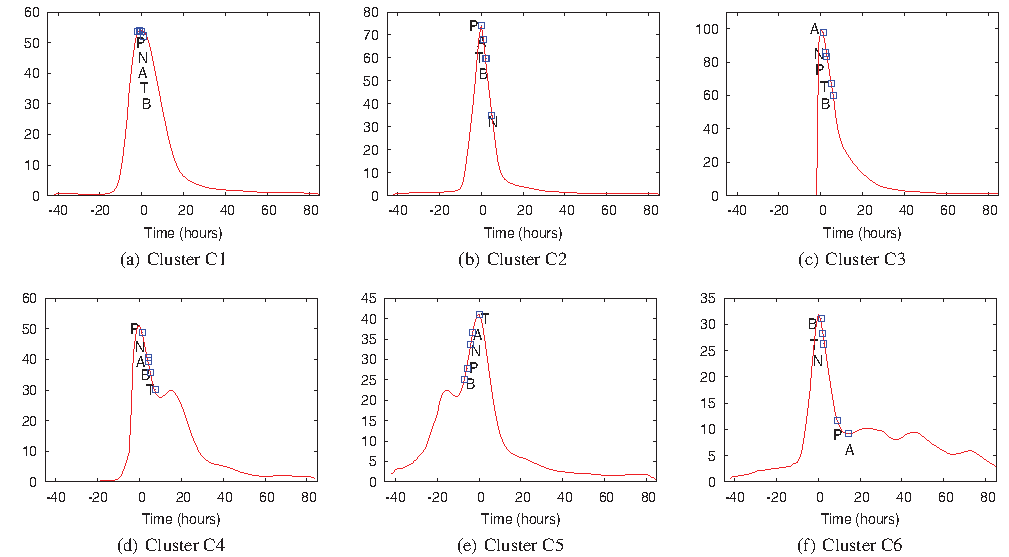
\includegraphics[width=0.8\textwidth]{pattern}
  \caption{Twitter平台中消息流行度变化的六种模式\citep{yang2011patterns}}
  \label{fig:pattern}
\end{figure}

流行度分布的不均匀性,以及增长过程出现的爆发现象和时序特性,吸引了大量研究人员的关注,进而涌现出了多种流行度预测的模型和方法。
\section{流行度预测方法概述}
现有的流行度预测方法主要包含三类:基于特征的有监督学习方法、基于随机过程的流行度到达过程建模方法和基于表示学习的方法。本节会依次对这三类方法进行介绍和总结。
\subsection{基于特征的有监督学习方法}
基于特征的流行度预测方法主要通过借助已有的有监督学习模型,结合人工抽取的特征,来对流行度的增长过程进行预测。在这类方法中,流行度预测问题通常会被形式化为分类或者回归问题:给定一组历史消息的各种特征信息以及消息在观测窗口$[0,T_r]$和预测窗口$[0,T_s]$内的流行度数据作为训练样本,利用现有的分类或回归方法学习得到预测模型,进而对待预测的消息的流行度作出预测。这类方法的核心在于寻找对于流行度预测有着重要指示作用的特征。常见的用于流行度预测的特征包括消息内容特征、用户特征、时序特征和传播级联的结构特征。

时序特征方面,常用于流行度预测的时序特征包括观测窗口内的累积流行度特征和流行度时间序列特征。Cha等人\citep{cha2009analyzing}分析了Youtube网站上视频的流行度增长数据,发现视频上传7天后的访问量和视频上传后一天以及上传后两天的访问量之间存在着非常强的相关性,进而提出了预测视频近期流行度的任务,并指出视频上传后短期内的累计流行度是重要的指示特征。Szabo等人\citep{szabo2010predicting}研究了Digg\footnote{\url{http://digg.com}}网站上的新闻数据和Youtube网站上的视频数据,发现这些内容早期的流行度和后期的流行度在进行对数变换后,存在着非常强的线性相关性,如图\ref{fig:loglinear}所示。基于这一观测,作者提出了S-H(Szabo-Huberman)模型,将消息在观测窗口内的累积流行度作为特征,利用对数线性回归模型来预测消息在预测时刻的流行度。Gursun等人\citep{gursun2011describing}分析了Youtube网站中部分视频在上传后一年内完整的观看频次序列,发现可以根据将视频按照访问频次分为两类:长期流行的视频和短期流行的视频,并利用时间序列分析模型中的自回归移动平均模型(Autoregressive Moving Average,ARMA)\citep{marple1987digital},对长期流行的视频的流行度变化过程进行了预测。
\begin{figure}[!htbp]
  \centering
  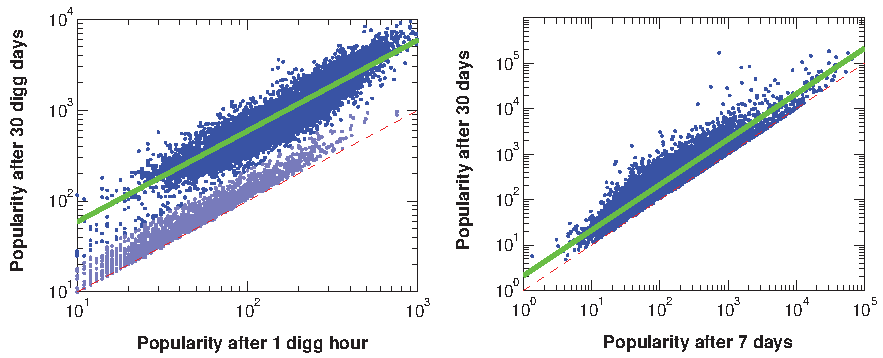
\includegraphics[width=0.9\textwidth]{loglinear}
  \caption{Digg平台和Youtube平台上早期流行度和后期流行度间的对数相关性\citep{sh2008Corr}}
  \label{fig:loglinear}
\end{figure}

Pinto等人\citep{pinto2013using}研究了Youtube网站中视频的流行度时间序列数据。作者将视频在观测窗口等分为若干长度相等的区间,并抽取了各时间区间内视频的观看数的增长量作为特征。作者在研究视频的时间序列后发现S-H模型的假设存在着局限性:早期累计流行度相近的视频,后期的流行度变化过程可能会有很大的差距,如图\ref{fig:pinto}所示。作者提出将消息在观测窗口内的时间序列数据作为特征,利用多元线性回归模型来预测消息的流行度。
\begin{figure}[!htbp]
  \centering
  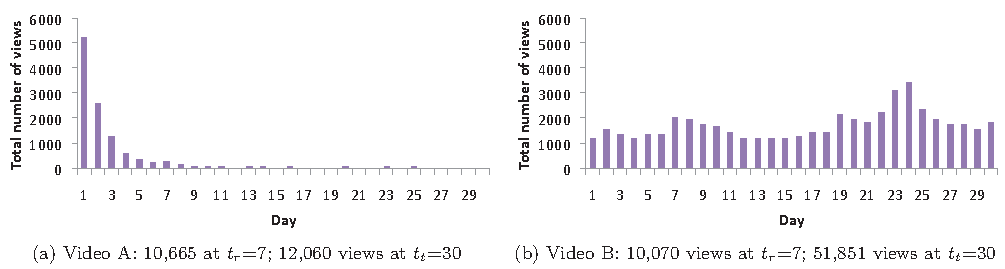
\includegraphics[width=1\textwidth]{pinto}
  \caption{S-H模型假设的局限性示例\citep{pinto2013using}}
  \label{fig:pinto}
\end{figure}

内容特征方面,Tsagkias等人\citep{tsagkias2009predicting}抽取了新闻的内容特征,来对新闻的评论数进行事前预测:在新闻发布之前,利用新闻的元信息,来预测新闻的评论数。作者将这一预测问题形式化为两阶段分类问题:新闻发布能否接收到评论,以及接收到的评论数会高还是低。在特征方面,作者抽取了新闻中重要性较高的前100个词的词频信息作为新闻的文本特征,新闻中包含的不同类型的命名实体的个数作为新闻的语义特征。此外,作者还抽取了新闻的其他元信息特征。实验结果表明,文本特征和语义特征对分类结果有较好的指示作用。Hong等人\citep{hong2011predicting}同样将Twitter平台中消息的流行度预测问题形式化为一个两阶段分类问题:消息是否会被转发以及消息最终的流行度等级。作者利用TF-IDF模型和LDA主题模型\citep{blei2003latent}来抽取消息的内容特征,同时结合网络拓扑结构特征以及时序特征来进行预测。Bandari等人\citep{bandari2012pulse}研究了新闻订阅站点Feedzilla\footnote{\url{http://news.feedzilla.com}}的数据在Twitter平台上的流行度情况。作者抽取了新闻的四类内容特征来进行预测,包括新闻所属的类别、新闻源站点的信息、新闻的倾向性特征和新闻中包含的命名实体。作者分别使用回归和分类模型对新闻的流行度进行了预测,得到了很好的预测效果。Bian等人\citep{bian2014predicting}研究了腾讯微博\footnote{\url{http://t.qq.com}}中消息的传播情况和用户的参与情况,从兴趣导向、社交影响和病毒式传播三个方面,建模了用户和消息之间的相互作用,进而对消息的流行度和用户的参与情况进行预测。建模过程中,作者提出了一种多任务迁移模型来建模消息的内容,提取出消息中的主题信息,用于后续的预测任务。

用户特征方面,最常见的用户特征是用户在社交网络中的拓扑结构信息,例如Twitter平台中用户的粉丝数和关注数信息\citep{gupta2012predicting,zhao2013short,kupavskii2013predicting,kong2014predicting}。用户的某些元信息也会被提取作为特征,包括用户账号的创建时长、用户历史发布的消息数\citep{suh2010want}、视频网站中的用户类别\citep{borghol2012untold}等。Yang等人\citep{yang2010modeling}在研究Twitter平台上消息的传播情况时,考虑了用户间的相互影响,提出了一种线性影响力模型。该模型可以在网络拓扑结构未知的情况下,来刻画用户间的影响力。Cui等人\citep{cui2013cascading}在研究Twitter平台上的消息爆发预测时,直接将用户身份作为特征。消息爆发预测问题旨在于给定消息在观测窗口内的流行度变化情况,预测消息最终的流行度能否达到爆发的阈值。作者在建模时借助于传感器的思想,将网络中所有的用户都当作传感器,只需要根据部分关键传感器的激活状态,即用户是否参与消息转发,就可以来判断消息最终能否爆发。因此,作者将爆发预测问题形式化为一个二分类问题,以所有的用户为特征,将用户在观测窗口内的激活状态转化成0-1向量作为输入,以消息最终的爆发情况作为输出,训练得到一个二分类器,进而对待预测的消息进行预测。

传播级联的结构特征方面,Bao等人\citep{bao2013popularity}分析了新浪微博中消息的传播级联情况,重点研究了传播级联形成的转发树的深度和链接密度情况,发现这两个特征与流行度的变化之间存在着非常强的相关性。作者将这两个因素加入到S-H模型中,发现预测精度得到了很大的提升。

除上述四类特征之外,研究人员还探寻了很多其他因素对流行度的影响。Brodersen等人\citep{brodersen2012youtube}研究了Youtube视频的观看数与地理因素之间的关系。Jenders等人\citep{jenders2013analyzing}研究了内容的情感倾向性对Twitter平台中消息转发数的影响。Weng等人\citep{weng2013virality}研究了流行度与网络的社区结构之间的关系,Junus等人\citep{junus2015community}也将社区结构因素建模到流行度预测模型中。此外,还有工作考虑了用户有限的关注度对流行度的影响\citep{hodas2012visibility,weng2012competition}。

问题形式化方面,不同于传统工作中将流行度预测形式化为一个回归或者分类问题,Cheng等人\citep{cheng2014can}将流行度预测问题形式化为阶段性的增长预测问题。作者指出,在以往的流行度分类预测问题中,由于流行度本身的分布是幂律的,导致各个类别样本数极度不均匀,从而影响最终的预测效果。因此,作者提出了``$kto2k$"问题:给定当前流行度为$k$的消息,预测它们最终的流行度能否增长到$2k$。基于样本集中流行度的分布,作者证明了提出的``$kto2k$"问题是一个均衡的二分类问题,并抽取了内容特征、用户特征、网络结构特征以及时序特征来进行预测。实验结果表明,随着$k$的增长,分类预测的准确率也在不断提高。

综上所述,基于特征的有监督学习方法在进行流行度预测时,关键在于抽取出能指示流行度变化的特征,但是特征工程是一项非常耗时耗力的工作,而且很大程度上受限于研究人员的先验认识。

\subsection{基于随机过程的流行度到达过程建模方法}
基于随机过程的流行度到达过程建模方法主要是在生存分析理论\citep{klein2005survival}的框架下进行的。这类方法中常见的流行度预测问题定义如下:给定一条消息$m$在观测窗口$[0,T]$内每一次转发的时间戳序列$C^m=\{t_i^m|0=t_0^m \le t_1^m \le...\le t_N^m \le T \}$作为输入,其中$N$表示消息$m$在观测窗口内总的转发次数,$t_i^m$表示消息$m$的第$i$次转发的转发时间与消息$m$的源发时间的间隔,最终的目标是预测后续流行度随时间的变化情况。这类方法通常将流行度的增长过程形式化为一个计数过程(Counting process)\citep{andersen1985counting}:用随机过程$\{N(t),t \ge 0\}$来刻画消息累积流行度随时间$t$变化的序列,其中$N(t)$取值是非负整数,且满足单调性:$N(s) \le N(t)\text{,} \forall s \le t$。在生存分析理论框架下,建模序列$N(t)$的关键在于对强度函数(Intensity function)的刻画。强度函数$x(t)$刻画了在给定历史信息$H_t=\{t_i|t_i < t \}$时,时间区间$[t,t+dt)$内有新事件发生的概率,即:
\begin{equation}
\label{eq:intensity}
P\{[t,t+dt)\text{内事件发生} | H_t\}=x(t)dt\text{。}
\end{equation}
用$dN(t)$来表示在时间区间$[t,t+dt)$内发生的事件数,它的期望可以用$\mathbb{E}_{dN(t) \sim \{0,1\}}[dN(t)|H_t]=x(t)dt$表示,从而可以得到计数序列$N(t)$与强度函数$x(t)$之间的关系如下:
\begin{equation}
\label{eq:differential}
\frac{\mathbb{E}[dN(t)]}{dt}=x(t)\text{。}
\end{equation}
在确定强度函数的形式和参数后,可以通过求解公式(\ref{eq:differential})中的微分方程,来确定计数序列$N(t)$的具体形式,进而对任意时刻$t$的计数值进行预测。

强度函数的形式通常由研究人员通过先验知识来确定,而具体的参数可以在生存分析理论框架下求取。生存分析理论常用于建模某一类事件发生的概率随时间的变化关系,例如患病病人的存活概率随时间的变化关系。在生存分析理论中,用随机变量$T$来表示事件发生的时刻,则概率$S(t)=P(T>t)$表示了事件到$t$时刻仍未发生的概率,因此被称为生存概率,而$F(t)=P(T \le t)=1-S(t)$则被称为累积死亡概率。累积死亡概率$F(t)$对应的密度函数$f(t)$可以通过如下求导的方式获得:
\begin{equation}
\label{eq:density}
f(t)=\frac{dF(t)}{dt}=\frac{P(t \le T < t+dt)}{dt}\text{。}
\end{equation}
在生存分析理论中,强度函数$x(t)$与密度函数$f(t)$的关系可以用如下公式表示:
\begin{eqnarray}
\label{eq:intensityTransform}
\begin{split}
x(t) & =\frac{P\{[t,t+dt)\text{内事件发生}|H_t\}}{dt}=\frac{P\{t \le T < t+dt|T \ge t\}}{dt} \\
& =\cfrac{\cfrac{P\{t \le T < t+dt\}}{P\{T \ge t\}}}{dt}=\cfrac{\cfrac{P\{t \le T < t+dt\}}{dt}}{P\{T \ge t\}}=\frac{f(t)}{S(t)}\text{。} 
\end{split}
\end{eqnarray}
将密度函数$f(t)$的定义$f(t)=F'(t)=(1-S(t))=-S'(t)$代入公式(\ref{eq:intensityTransform}),可以得到:
\begin{equation}
\label{eq:intensityDifferential}
x(t)=\frac{f(t)}{S(t)}=-\frac{S'(t)}{S(t)}=-\frac{d[lnS(t)]}{dt}\text{。}
\end{equation}
两边取积分,得到:
\begin{equation}
\label{eq:intensitySurvival}
S(t)=exp\{-\int_{0}^{t}x(t)dt\}\text{。}
\end{equation}
密度函数$f(t)$也可以通过如下公式由强度函数$x(t)$来表示:
\begin{equation}
\label{eq:intensityDensity}
f(t)=x(t)\ast S(t)=x(t) \ast exp\{-\int_{0}^{t}x(t)dt\}\text{。}
\end{equation}
由此可见,在生存分析理论框架下,事件发生的概率密度和生存概率都可以用强度函数表示出来。在给定观测数据后,可以通过极大似然估计的方式,求取强度函数中的参数,得到强度函数的具体形式。具体到流行度预测问题中,对于前述给定的时间戳序列$C^m$,可以定义它的似然函数如下:
\begin{equation}
\label{eq:likelihood}
\mathcal{L}\{C^m\}=P_0(T|t_N^m)\prod_{i=1}^{N}p_1(t_i^m|t_{i-1}^m)\text{,}
\end{equation}
其中$P_0(T|t_N^m)$刻画了从$[t_N^m, T]$时间区间内没有新的流行度到达的概率,$p_1(t_i|t_{i-1})$刻画了给定上一次转发时刻为$t_{i-1}^m$的情况下,下一次转发发生在$t_i^m$的概率。在生存分析理论框架下,这两个概率分别对应$[t_N^m, T]$区间内的存活概率和$t_i^m$时刻的概率密度。给定强度函数$x(t)$,这两个概率可以如下表示:
\begin{eqnarray}
\label{eq:eventProb}
\begin{split}
P_0(T|t_N^m) & =exp\{-\int_{t_N^m}^T x(t)dt\}\text{,}\\
p_1(t_i^m|t_{i-1}^m) & =x(t)\ast exp\{-\int_{t_{i-1}^m}^{t_i^m} x(t)dt\}\text{。}
\end{split}
\end{eqnarray}
因此,在给定序列$C^m$的情况下,结合公式(\ref{eq:likelihood})和公式(\ref{eq:eventProb}),就可以求出强度函数$x(t)$的具体形式,进而根据公式(\ref{eq:differential})对流行度后续增长情况做出预测。

鉴于计数过程和流行度增长过程的天然相似性,很多流行度预测的工作都是从随机过程的角度开展的。Wang等人\citep{wang2013quantifying}研究了论文的引用数增长情况。作者提出并论证了影响论文引用数增长的三个关键因素:论文本身的质量、论文自身吸引力的时效性以及论文累积引用数,并将这三个因素建模到论文引用数的增长过程中。作者提出的模型可以根据论文发表后10年内的引用信息,来预测后续20年论文引用数的增长情况。在该工作的基础上,Shen等人\citep{shen2014modeling}采用了自增强泊松过程(Reinforced Poisson process, RPP)\citep{pemantle2007survey}来建模论文的引用数增长情况。在建模引用序列的强度函数时,作者考虑了上述三个影响因素,给出如下的强度函数:
\begin{equation}
\label{eq:intensityRPP}
x(t)=\lambda f(t;\theta)i(t)\text{,}
\end{equation}
其中$\lambda$是对论文本身质量的度量;$f(t;\theta)$是一个时序释放函数,用于刻画论文的吸引力随时间的变化情况,$\theta$是时序释放函数的参数;$i(t)$是自增强函数,用于刻画论文引用中的``富者愈富"现象。在论文引用数据集上,作者选取了Log-normal函数作为时序释放函数,并将自增强函数$i(t)$定义为到$t$时刻为止的论文引用数。数据集上的实验结果表明,作者提出的自增强泊松过程模型(RPP模型)可以很好地刻画论文引用的到达过程。此外,作者还对模型中的参数引入了先验,进一步提升了模型的预测效果。Gao等人\citep{gao2015modeling}将RPP模型应用到微博平台上消息的转发数预测中。作者详细分析了微博平台中消息转发数据的特点,并对RPP模型中的时序释放函数和自增强函数的形式进行了相应的修正。此外,作者还分析了微博平台中时间的异质性,引入``微博时间"的概念来对微博平台中的物理时间进行映射,从而消除时间异质性对预测效果的影响。修正后的RPP模型在微博转发数预测任务上取得了非常好的效果。

Bao等人在\citep{bao2015modeling}中指出,RPP模型在建模过程中,是将消息传播当做一个单源传播的过程,没有考虑转发操作带来的激励作用,这样的建模方式不适用于微博平台上的转发数据,因为微博平台中用户间的转发行为会影响消息最终的转发数。因此,作者提出利用自激励Hawkes过程(Self-exciting Hawkes process, SEHP)来建模每次转发带来的激励作用。基于自激励Hawkes过程,作者提出了如下强度函数:
\begin{equation}
\label{eq:hawkesIntensity}
x(t)=v e^{-\beta t}+\alpha \sum_{j=1}^{j_{max}(t)} e^{-\beta(t-t_j)}\text{,}
\end{equation}
其中,$j_{max}(t)$刻画了到$t$时刻为止的转发次数,$v$是对消息本身吸引力的度量,$\alpha$刻画了每次转发带来的激励强度,函数$e^{-\beta t}$刻画了激励强度随时间的衰减效应。相比于RPP模型,SEHP模型能更好地捕获每次转发带来的影响,如图\ref{fig:sehp}所示。在该工作的基础上,作者还提出了ISEHP模型\citep{bao2016modeling},进一步考虑了不同转发用户带来的激励强度的差异以及微博平台上的时间异质性。
\begin{figure}[!htbp]
  \centering
  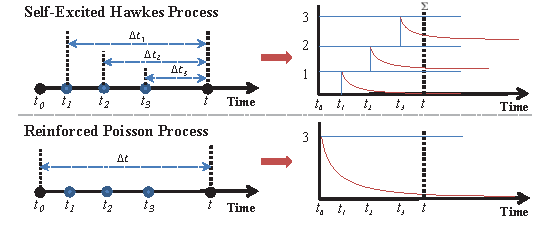
\includegraphics[width=0.75\textwidth]{sehp}
  \caption{SEHP模型和RPP在刻画激励作用时的差异\citep{bao2015modeling}}
  \label{fig:sehp}
\end{figure}

Zhao等人\citep{zhao2015seismic}研究了社交网络中消息爆发预测的问题。作者将爆发预测问题形式化为消息最终流行度的预测问题。作者同样采用了自激励Hawkes过程来建模消息流行度的转发过程。在建模用户激励强度时,作者引入了用户粉丝数,同时还将消息本身的感染力也建模成一个随机过程。最终作者给出流行度增长过程的强度函数如下:
\begin{equation}
\label{eq:seismic}
x(t)=p(t) \sum_{t_i<t}n_i \phi(t-t_i)\text{,}
\end{equation}
其中$p(t)$是用于刻画消息自身感染强度变化的随机过程,$n_i$是第$i$转发的用户的粉丝数,$\phi(t-t_i)$用于刻画感染强度随时间的变化关系。作者在论文中还指出,感染强度$p(t)$的大小反映了消息当前所处的增长状态:令$n^{\ast}$表示所有用户的粉丝数的平均值。当$p(t)>1/n^{\ast}$时,消息处于``超临界"状态,此时消息的流行度处于指数增长阶段,无法对消息的最终流行度做出预测;当$p(t)<1/n^{\ast}$时,消息处于``次临界"状态,此时消息的流行度增长状态逐渐减缓,可以预测消息的最终流行度。

在自增强泊松过程和自激励Hawkes过程以外,也有一部分工作采用了其他的随机过程来刻画流行度的增长情况。Lerman等人\citep{lerman2010using}研究了Digg网站上故事的得票数的变化情况。分析发现,故事在网站中的曝光度、故事本身的内容吸引力以及用户间的社会关系对故事最终的得票数有很大的影响。作者将这三个因素建模到故事得票数增长模型中,得到了很好的预测效果。Costa等人\citep{ferraz2015rsc}分别使用了使用泊松过程(Poisson process)\citep{kingman1993poisson}和自相关过程(Self-correlated process)来建模了消息的转发时间间隔的产生过程。Yang等人\citep{yang2013mixture}采用了多元Hawkes过程来建模多条消息的转发情况。Rizoiu等人\citep{rizoiu2017expecting}提出了Hawkes强度过程(Hawkes intensity process,HIP)来建模流行度时间序列的产生过程。Yu等人\citep{yu2015micro}研究了微博平台中消息的微观转发过程,并直接使用了生存分析理论来建模平台中用户发布的消息被自己的粉丝转发的概率。

纵观上述方法,基于随机过程的方法能够较好地刻画流行度的到达过程,但是由于是非监督学习的方法,它们的预测能力有限;同时流行度增长的强度函数的设计,很大程度上也依赖于研究人员的先验知识;另外,这类方法在建模过程中只利用了待预测消息自身的信息,没有显式地利用海量的历史消息来辅助提升预测性能。

\subsection{基于表示学习的方法}
表示学习目前已经发展成为一个重要的领域,在很多实际问题中都有着重要的应用。在流行度预测领域,Bourigault等人\citep{bourigault2014learning}通过学习用户表示来预测消息的传播过程。作者将消息的传播过程类比为一个热传导的过程:消息的发布者作为``热源",距离用户越近的用户,会越早地参与到热传导中来。因此,作者将所有的用户都嵌入到一个隐空间中,用户参与消息转发的先后顺序由用户与消息源发用户在隐空间中的距离决定。借助排序的框架,作者根据数据集中用户参与转发的先后顺序,学习得到所有用户的表达,并根据当前的转发情况,对接下来参与转发的的用户进行预测。Liu等人\citep{liu2016learning}在该工作的基础上,考虑了用户作为发布者和转发者的区别,为每个用户分别学习了影响力表达和易感性表达,并进一步建模了用户参与转发的先后顺序上的差异。此外,Bourigault等人\citep{bourigault2016representation}还在独立级联模型\citep{goldenberg2001talk}中引入用户表示学习,来建模消息的转发过程。

在深度学习领域,以循环神经网络(Recurrent neural network,RNN)\citep{mikolov2010recurrent}和带长短时记忆单元(Long-short term memory,LSTM)\citep{hochreiter1997long}以及门控循环单元(Gated recurrent unit,GRU)\citep{cho2014learning}的循环神经网络为代表的模型在语音识别、文本生成等一系列序列建模领域都取得了突破性的成果。流行度的增长过程本身也是一个转发事件序列不断生长的过程,因此,这类序列建模的方法也可以用来建模流行度序列的增长过程。Du等人\citep{du2016recurrent}在建模带标记的事件序列时,在随机点过程的框架下,用RNN网络来建模事件序列的强度函数。作者在论文中指出,传统的基于随机过程的方法都需要人工去定义强度函数的形式,而人工定义的函数形式与真正的强度函数可能相去甚远,导致模型的预测能力下降。
因此,作者提出了RMTPP模型,使用RNN网络来建模传播过程中强度函数的变化,模型的整体结构如图\ref{fig:rmtpp}所示。
\begin{figure}[!htbp]
  \centering
  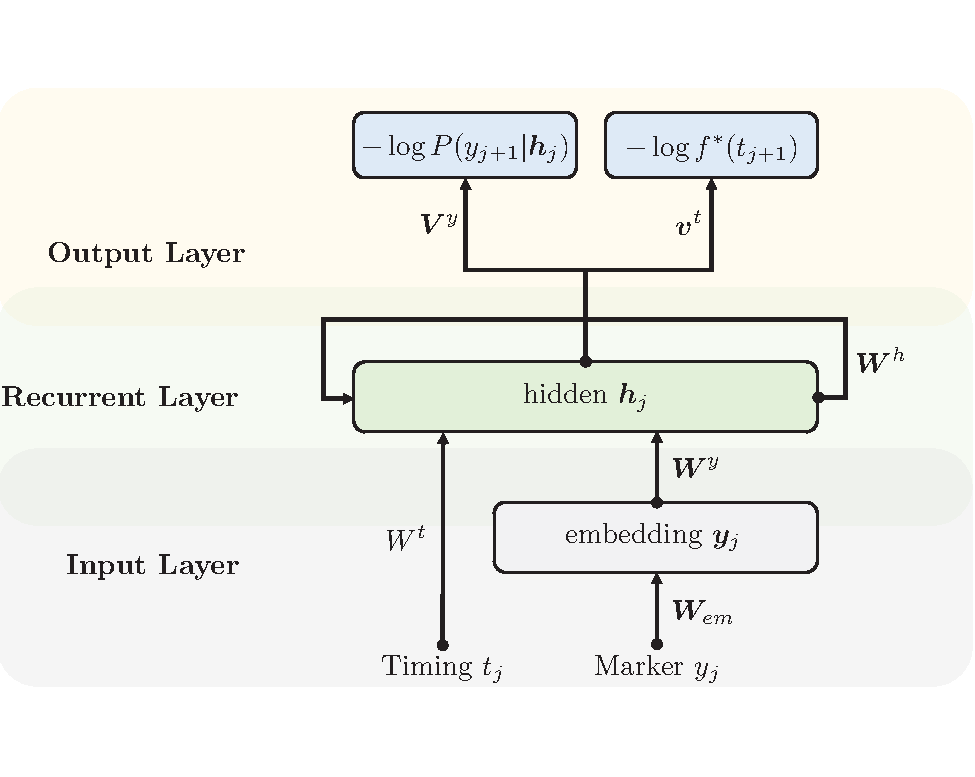
\includegraphics[width=0.5\textwidth]{rmtpp}
  \caption{RMTPP模型的结构示意图\citep{du2016recurrent}}
  \label{fig:rmtpp}
\end{figure}
该模型以事件发生时刻和事件类型作为输入,利用RNN网络来学习历史事件集合的表达,在历史事件表达的基础上计算得到事件的累积强度函数,并对下一次事件的发生时刻和类型做出预测。
Wang等人\citep{wang2017marked}在该工作的基础上,引入了事件发生时刻和事件类型之间的依赖关系,进一步提升了模型的预测效果。Xiao等人\citep{xiao2017modeling}也采用了RNN网络来建模消息的强度函数。在建模过程中,作者将强度函数分解成历史转发激励和消息固有的传播能力两部分,分别使用了两个RNN网络来建模消息的转发时刻序列和流行度时间序列,再将两个RNN网络的结果融合得到消息传播强度的表示。
\begin{figure}[!htbp]
  \centering
  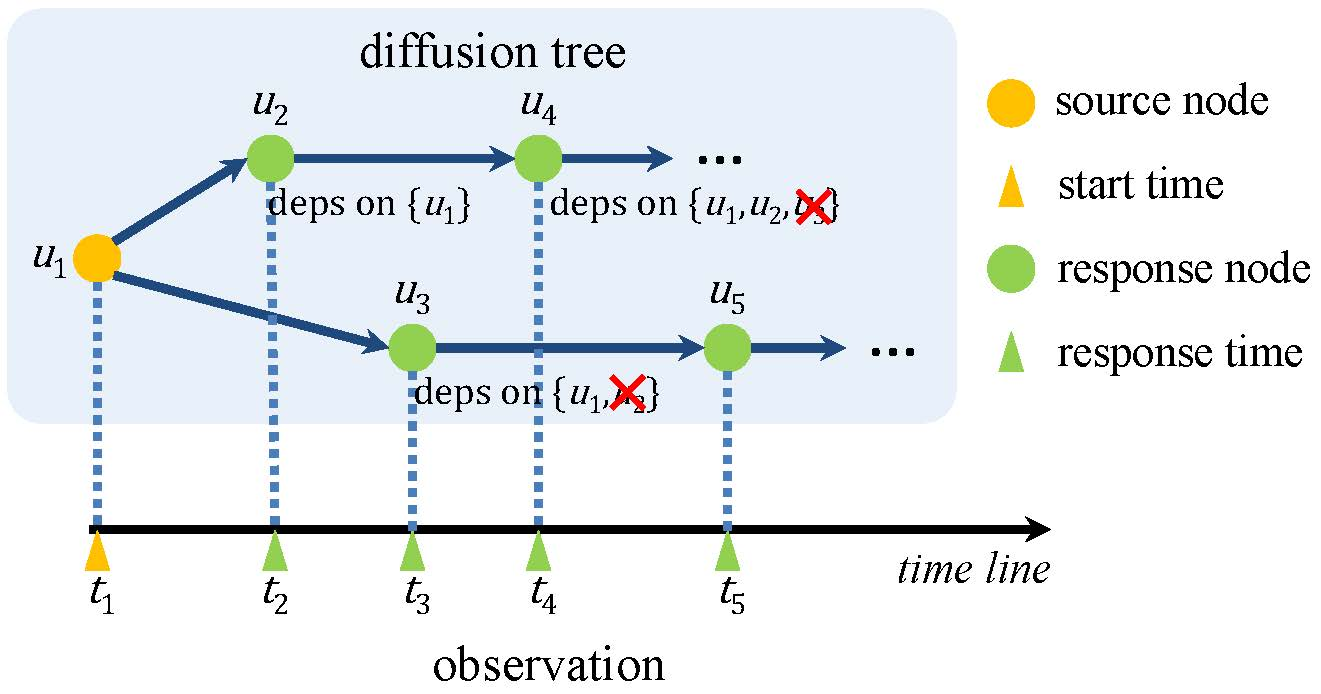
\includegraphics[width=0.5\textwidth]{crossDependence}
  \caption{消息传播过程中的跳跃依赖现象\citep{wang2017cascade}}
  \label{fig:crossDependence}
\end{figure}

尽管以RNN网络为代表的模型在流行度建模领域取得了一定的成果,Wang等人\citep{wang2017cascade}在论文中指出:RNN网络可以建模序列中的顺序依赖关系,但是很难处理消息转发过程中存在的``跳跃依赖"。消息转发过程中的跳跃依赖如图\ref{fig:crossDependence}所示。在图示的转发过程中,用户$u_3$的行为只依赖于$u_1$,而不依赖与$u_2$;同理用于$u_4$的转发行为依赖于$\{u_1,u_2\}$,而不依赖于$u_3$。传统的RNN网络无法建模这类跳跃依赖问题。因此,作者在RNN网络中的基础上,引入了关注机制\citep{bahdanau2014neural}来学习传播过程中更精确的依赖关系。

除上述基于用户表示学习的模型和深度序列模型外,还存在一部分基于深度模型的``端到端"的流行度预测方法。Li等人\citep{li2017deepcas}提出了DeepCas模型在对消息的流行度进行预测。DeepCas模型从消息的转发树结构出发,利用随机游走\citep{spitzer2013principles}的方式从转发树中采样得到若干转发序列;再利用带GRU单元的双向RNN网络学习得到转发序列的表达;再利用权重机制将这些序列的表达融合得到消息的表达;最后利用一个多层神经网络来学习消息的表达和消息的流行度之间的变换关系。DeepCas模型的整体结构如图\ref{fig:deepCas}所示。
\begin{figure}[!htbp]
  \centering
  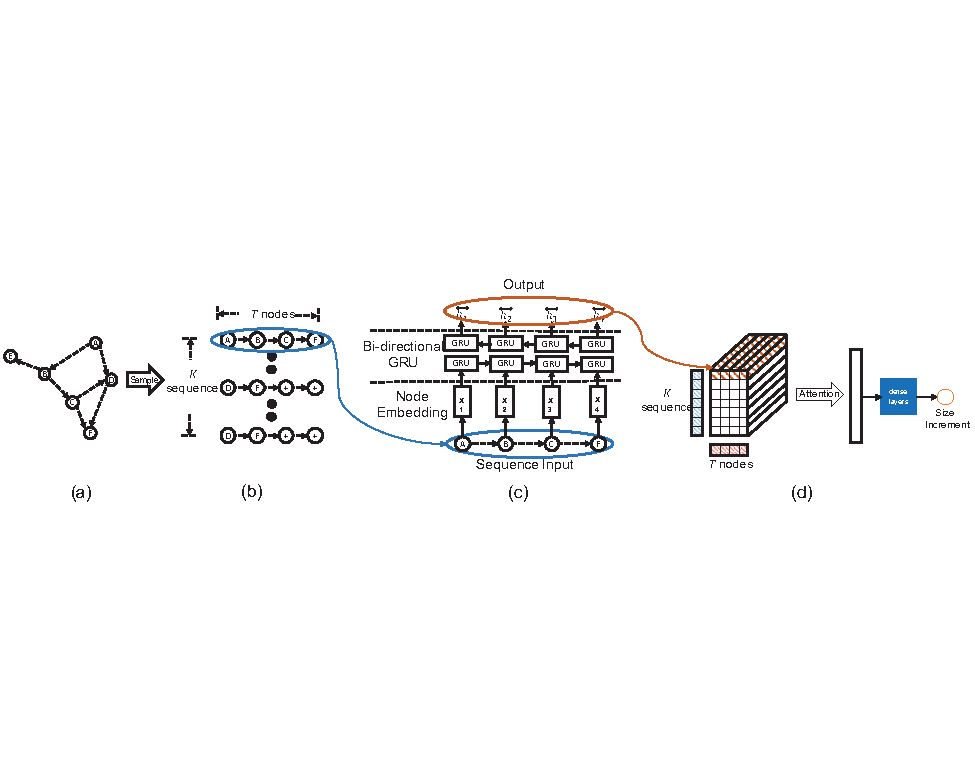
\includegraphics[width=1\textwidth]{deepCas}
  \caption{DeepCas模型结构示意图\citep{li2017deepcas}}
  \label{fig:deepCas}
\end{figure}
\begin{figure}[!htbp]
  \centering
  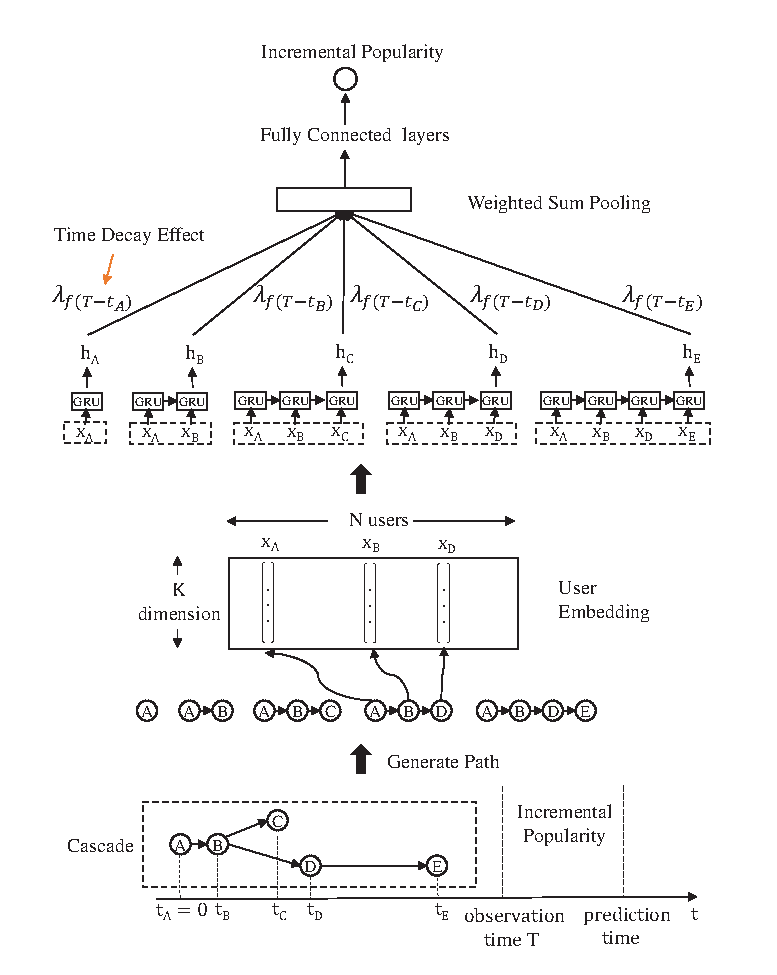
\includegraphics[width=0.52\textwidth]{deepHawkes}
  \caption{DeepHawkes模型结构示意图\citep{cao2017deep}}
  \label{fig:deepHawkes}
\end{figure}

Cao等人\citep{cao2017deep}从自激励Hawkes过程中受到启发,将影响消息流行度的三个关键因素:用户影响力、每次转发带来的激励效应以及激励的时间衰减效应分别用深度模型来建模,提出了DeepHawkes模型。DeepHawkes模型也是从消息的转发树出发,抽取出消息转发树中的所有路径,再利用深度序列模型对所有的路径进行建模,最后根据每条路径中尾节点的参与时间对路径的表达进行加权,得到消息的最终表达。消息的表达与消息的流行度之间的变换函数是通过一个全连接的神经网络学习得到。DeepHawkes模型的整体结构如图\ref{fig:deepHawkes}所示。

\subsection{其他方法}
在上述三类方法外,还有一些工作从不同的角度来尝试对消息的流行度做出更精确的预测。Mishra等人\citep{mishra2016feature}提出了一种结合特征类方法和随机过程类方法的模型。作者先利用自激励Hawkes过程学习得到消息自身的吸引力、转发用户的影响力以及时间衰减效应的参数,然后将这三部分因素作为特征,与人工提取的特征一起,利用监督学习的框架,来预测消息最终的流行度。实验结果表明,作者提出的模型的预测效果要明显优于特征类方法和随机过程类方法的效果。Xiao等人\citep{xiao2016modeling}同样从融合特征类方法和随机过程类方法的角度,提出了一种新方法来预测论文的引用数。作者在自激励Hawkes过程的框架下,将论文自身的吸引力用一系列人工提取的特征来表示,对应的强度函数如下:
\begin{equation}
\label{eq:citationIntensity}
x(t)=[\boldsymbol{\beta} \boldsymbol{\psi}(t)]e^{-w_1 t}+\alpha \sum_{t_i<t}e^{-w_2(t-t_i)}\text{,}
\end{equation}
对比公式(\ref{eq:hawkesIntensity}),可以看到用于表示论文自身吸引力的变量由$[\boldsymbol{\beta} \boldsymbol{\psi}(t)]$替代,其中$\boldsymbol{\psi}(t)$是人工提取的指示特征向量,$\boldsymbol{\beta}$是待学习的相关系数向量。数据集上的结果表明,融合后的模型比随机过程类方法有着更好的预测效果。

另一部分工作从分组的角度来考虑流行度预测问题。Cao等人\citep{cao2017predicting}按照观测窗口内的累积流行度,将消息分到不同的组中;再分别用每个组别的数据去训练S-H模型发现不同组别学习得到的S-H模型的参数存在很大的差异性,说明了分组的必要性。Ouyang等人\citep{ouyang2016peek}在预测在线视频的流行度时,也采用了分组预测的思想。
\begin{figure}[!htbp]
  \centering
  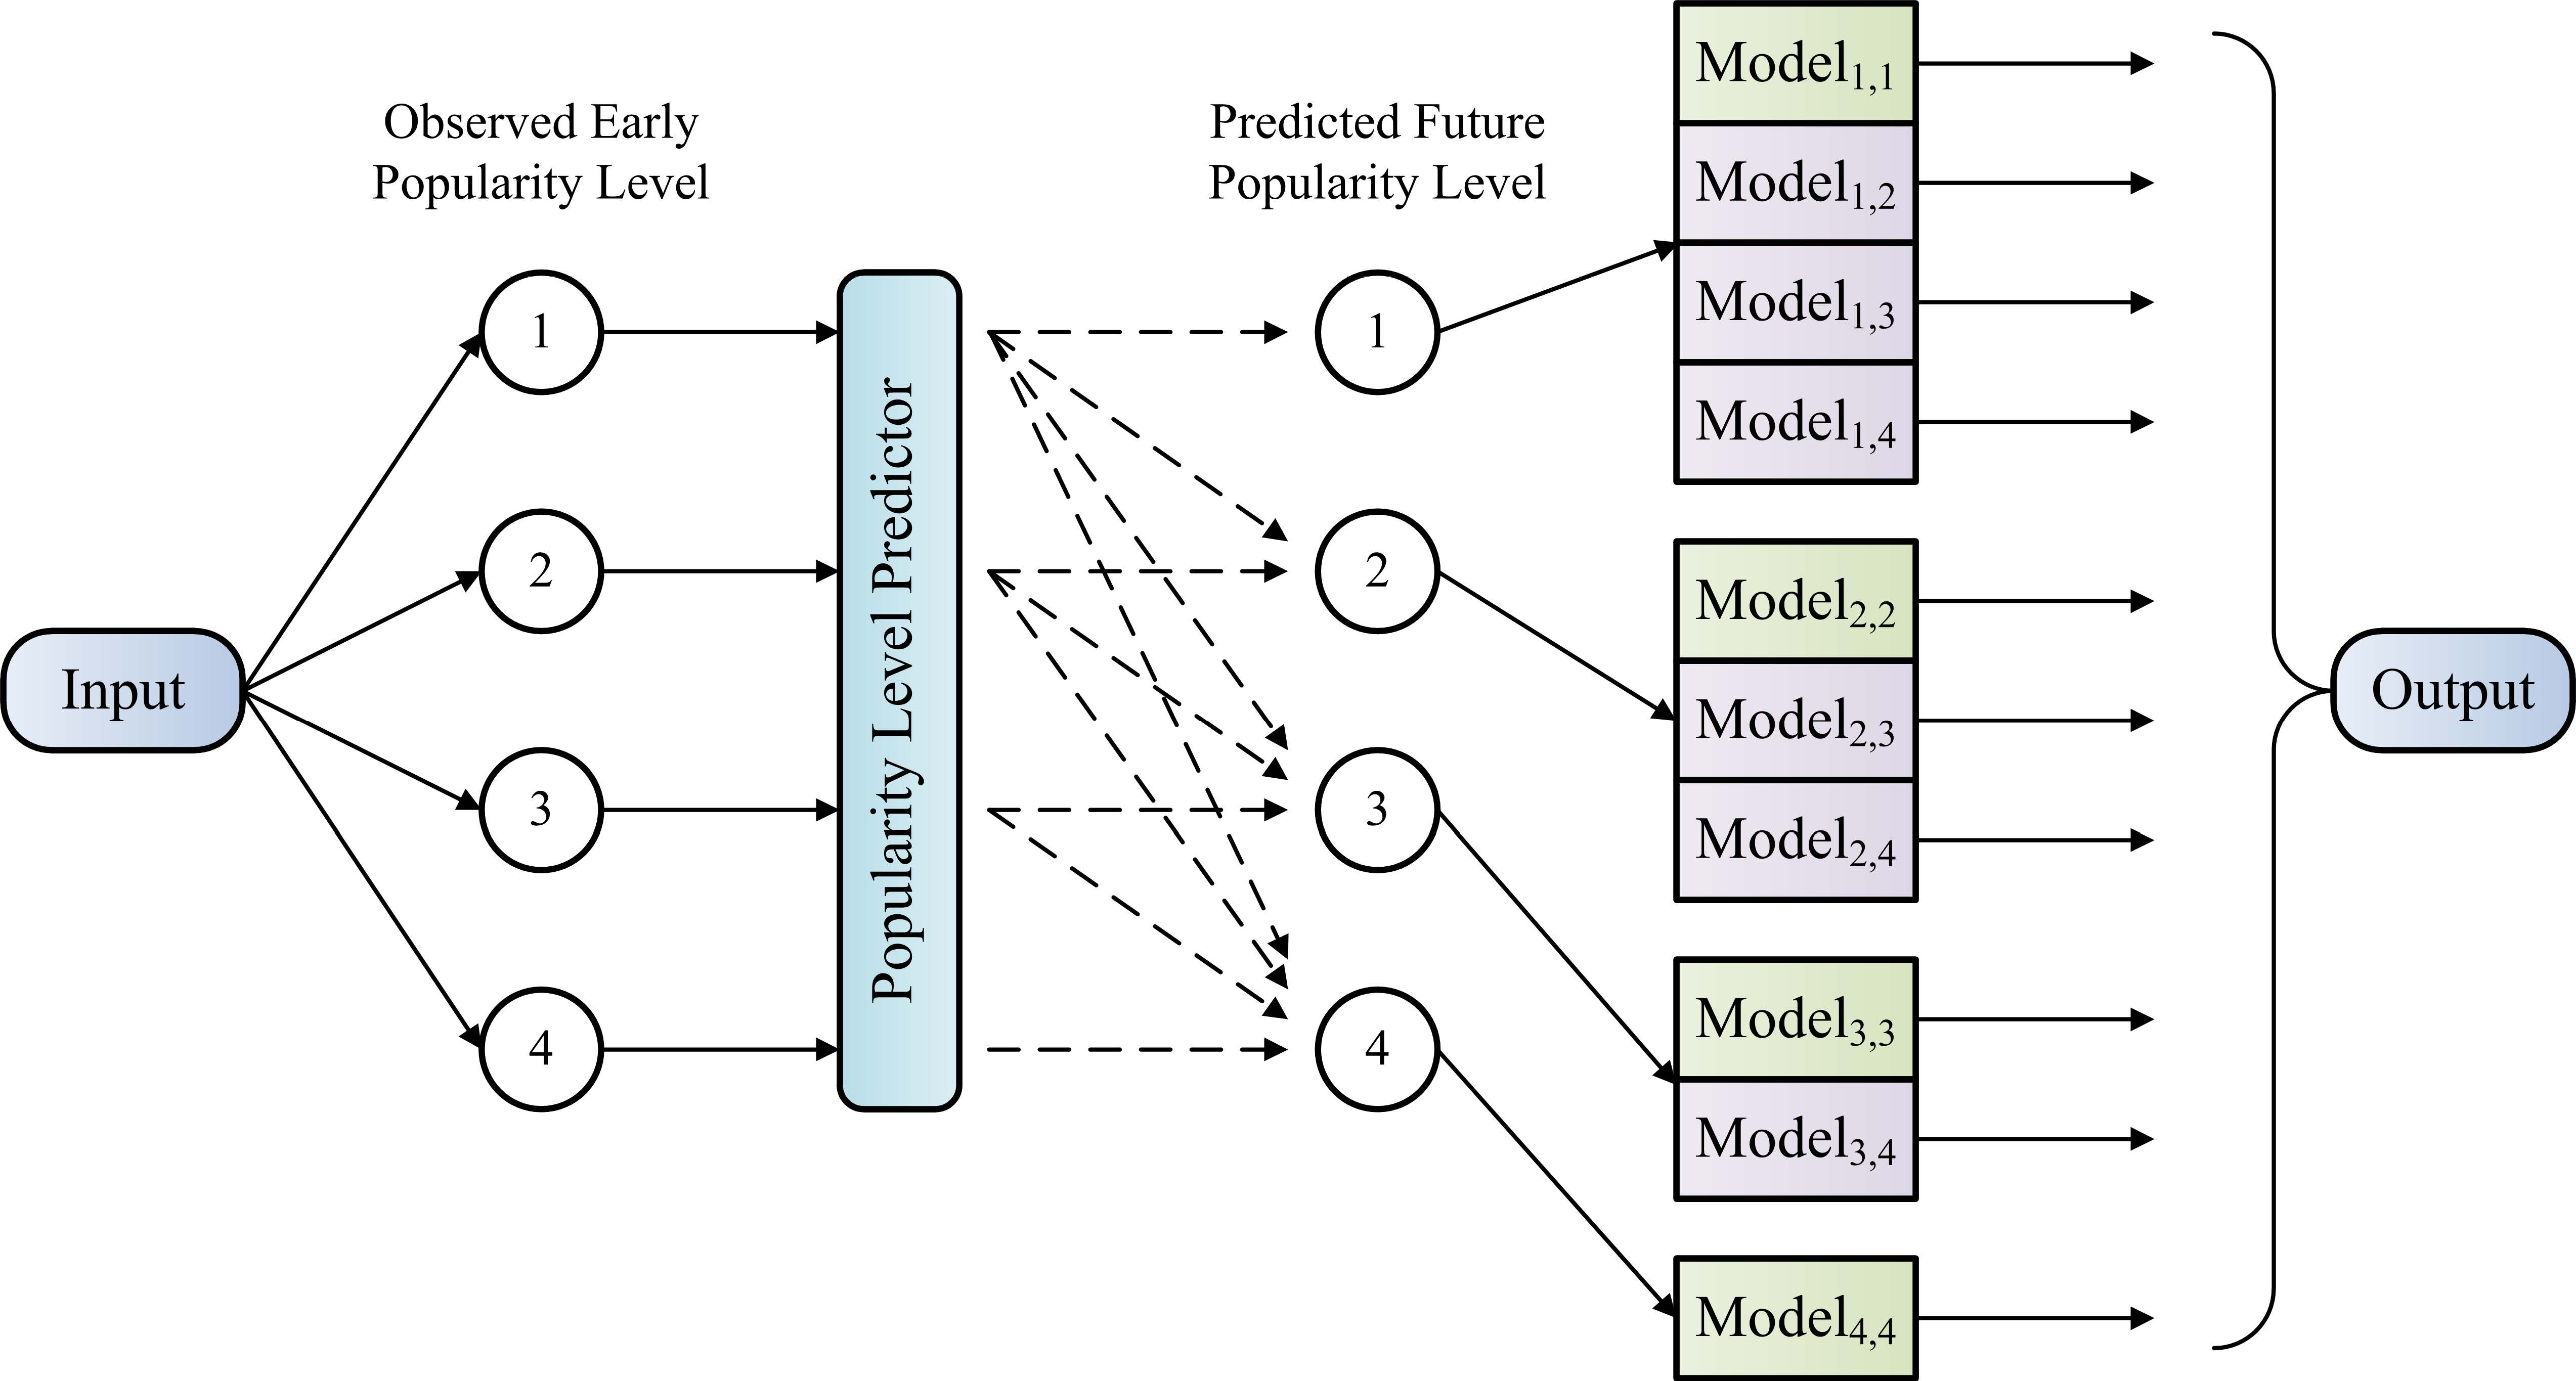
\includegraphics[width=0.45\textwidth]{peek}
  \caption{Ouyang等人提出的基于消息分组的流行度预测模型\citep{ouyang2016peek}}
  \label{fig:group}
\end{figure}作者将视频流行度预测问题分解为两个预测任务:预测视频最终流行度的级别以及预测视频最终流行度的数值。作者先提取了一些列的特征,来预测视频最终流行度的级别;再根据视频$v$在观测窗口的流行度级别$L_v(i)$和预测得到的最终流行度级别$L_v(r)$,分别利用不同的模型来预测视频最终的流行度:若$L_v(i)=L_v(r)$,说明视频最终流行度级别与观测窗口内的流行度级别相同,这种情况视频最终的流行度由观测窗口内的流行度变化趋势来决定,因而采用了Pinto模型\citep{pinto2013using}来预测;若$L_v(i)<L_v(r)$,说明视频最终的流行度得到了较大的提升,这种情况下作者采用了S-H模型来进行预测。预测方法的整体框架如图\ref{fig:group}所示。除消息分组的思想外,Hoang等人\citep{hoang2017gpop}还提出了基于用户分组的流行度预测方法。作者在论文中指出,现有的流行度预测方发主要从两个层面开展:用户层面,预测单个用户是否会参与转发;群体层面,预测最终会参与转发的用户总数。但用户层面的预测模型常常受到数据稀疏性的影响,而群体层面的预测模型又忽略了用户层面的特征。因此,作者提出一个基于用户分组的流行度预测方法。作者先根据用户所处的社交网络的结构和历史上参与消息转发的情况,将用户划分为不同的用户组;再将同一个组中用户的转发数据合并,得到用户组级别的转发数据;最后在合并后的``消息-用户-时间"数据上,利用张量填充\citep{Kolda2009TDA}的方式对待预测消息的流行度做出预测。

此外,还有部分工作考虑了传统过程中消息间的竞争与合作机制。Zarezade等人\citep{zarezade2017correlated}研究了Twitter平台上不同消息的传播情况,发现同时在传播的消息之间存在着竞争和合作的现象:处于竞争状态的消息的流行度呈现出此消彼长的变化趋势,而处于合作状态的消息的流行度则呈现出同步变化的趋势,如图\ref{fig:cooperate}所示。作者基于自激励Hawkes过程,引入消息间的竞争合作机制,较好地捕获了处于不同状态的消息的流行度的变化趋势。Samanta等人\citep{samantalmpp}同样在自激励Hawkes过程中引入了合作竞争机制来刻画Twitter平台上不同话题标签的流行度的变化情况。在考虑话题标签间的竞争机制时,作者引入了排序的思想,来对消息的强度函数进行约束。
\begin{figure}[!htbp]
  \centering
  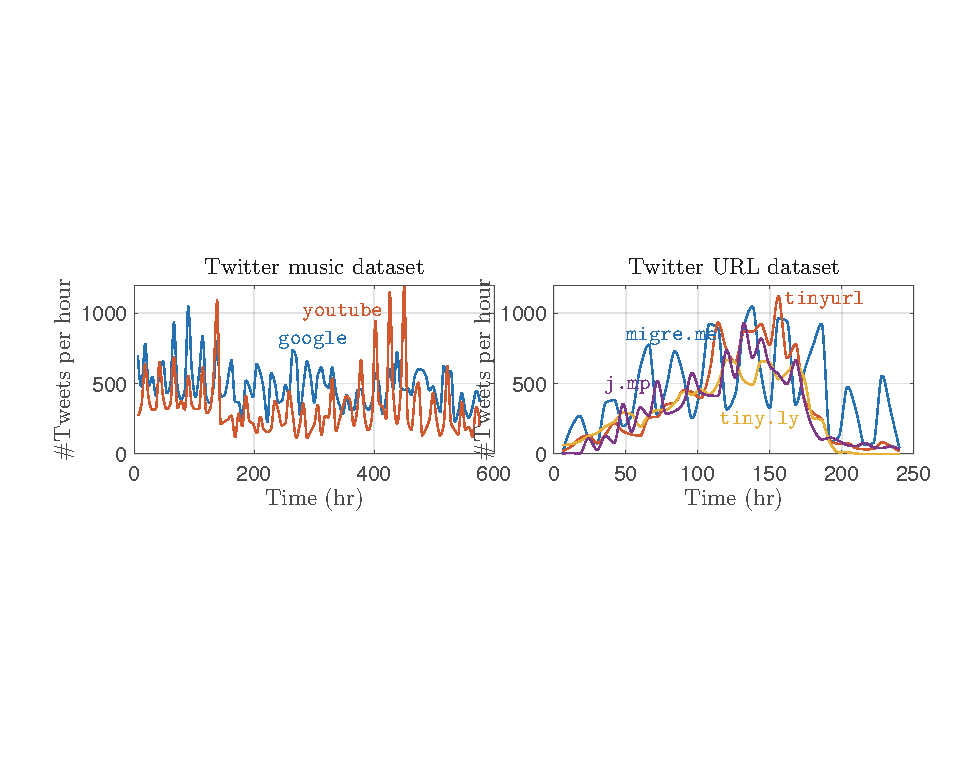
\includegraphics[width=0.75\textwidth]{compete}
  \caption{Twitter平台中消息间竞争合作示例\citep{zarezade2017correlated}}
  \label{fig:cooperate}
\end{figure}

总体来说,现有的流行度预测方法非常丰富,各类方法都有着自身的出发点和适用场景,但同时也都存在着不同程度的缺陷和不足,这也说明了流行度预测问题本身的难度非常大。

\section{流行度的可预测性分析}
在线社交网络中,内容的传播受多方面因素的影响,包括用户兴趣、网络拓扑结构、社交影响等。这些因素不仅使得内容的流行度分布表现出不均匀性,也使得内容的流行度预测变得非常困难,这也激发了研究人员对流行度的可预测性的研究和分析。Salganik等人\citep{salganik2006experimental}设计了一组实验,验证了社交网络中用户间的社交影响力确实会增加内容流行度的不可预测性。作者设计了一个虚拟的``音乐市场",在市场中提供了若干首未发布的音乐曲目。当用户进入到音乐市场后,可以点击听取音乐曲目的内容,并对曲目进行打分。此外,用户还可以下载喜欢的曲目。作者将每首曲目的下载次数作为它的流行度度量。为了体现社交影响力对流行度的影响,作者将用户分成不同的组别:对照组的用户只能看到曲目信息,而实验组的用户可以看到曲目当前的下载次数。最终的实验室结果发现,实验组中曲目的流行度的分布体现出更大的不均匀性,而且拥有着更高的不可预测性。两个组别的实验结果上的差异表明,社交影响力确实会增加曲目流行度的不可预测性。作者在文章中还指出,文中设计的虚拟实验只考虑了最简单的社交影响因素,即每首曲目当前的累计下载次数,而在实际的的传播系统中,各种因素的影响使得消息的传播数据拥有着更高的不可预测性。

Martin等人\citep{martin2016exploring}研究了复杂社交系统中成功的可预测性。作者以Twitter平台中消息传播数的``事前预测"为示例展开了消息。消息传播树的``事前预测"是指仅利用消息在发布之前的元信息进行预测。作者抽取了一系列的特征来进行预测。实验结果发现,尽管考虑了丰富的特征,预测模型的预测能力仍然存在着上界,这说明社交系统中的消息传播数预测问题本身存在上界。因此,作者提出了一种传播模拟模型,来从理论层面对这一上界进行了分析。实验结果表明,即使预测人员对系统的初始条件有着精准的估计,由于传播过程的复杂性,最终的预测结果仍然存在上界,而且系统中消息的质量分布越宽泛,系统整体的可预测性的上界就越低。此外,作者还发现,系统的可预测性的上界对初始条件非常敏感:只要在对初始条件的估计中出现微小的偏差,就有可能导致系统的可预测性上界出现大幅度的下滑。尽管作者在文中提出的传播模拟模型与真实社交网络中的传播相比,显得非常简单,但是作者得出的结论对社交网络中内容流行度的可预测性有重要的指导意义。

Shulman等人\citep{shulman2016predictability}分析了流行度预测问题的可预测性和可解释性之间存在的鸿沟。作者采用了\citep{cheng2014can}中的问题形式化定义:给定当前流行度为$k$的消息,预测它们最终的流行度能否达到$2k$。作者提取了一系列的特征进行了实验,发现基于时序特征的方法的预测效果要明显优于基于其他特征的方法,而且在不同的数据集上都表现出了较好的鲁棒性。同时,作者在文中指出,时序特征虽然在预测效果上有较好的表现,但是从可解释性的角度,它的意义非常有限,因为时序特征并不能解释消息间流行度差异的原因。

2017年2月,《科学》杂志推出了一起关于预测问题的专栏\citep{Jasny468},Hofman等人在该专栏中发表文章\citep{hofman2017prediction},以Twitter平台中消息的转发数预测为例,阐述了目前预测领域的存在一些问题:首先是预测问题的标准化。目前的预测问题的形式化多种多样,采用的数据集和评价指标也各不相同,这种现象无疑限制了预测领域的发展;其次是对问题的可预测性要有精准的刻画,以便于了解模型的预测效果的期望值;最后模型的预测效果和可解释性应该是互补的关系,而不是互相替代的关系。

总体来说,社交网络中内容的流行度受多方面因素的影响,问题本身的可预测性也因为多种影响因素的存在,很难被精确的刻画。社交网络是一个非常复杂的系统,其中传播的内容的流行度预测是一个很难的问题。

\section{本章小结}
本章主要对流行度预测领域的工作进行了介绍和总结,包括流行度的统计特征分析、现有的流行度预测方法以及流行度本身的可预测性。统计特征分析方面,社交网络中内容的流行度都呈现出幂律分布,在传播过程中存在着爆发现象,并且呈现出了固定的传播模式。流行度预测方法方面,主要介绍了基于特征的方法、基于随机过程的方法以及基于表示学习的方法。此外,文中还介绍了部分提高预测性能的策略,包括融合特征类方法和随机过程类方法、消息分组和用户分组策略以及考虑消息传播过程中的竞争合作机制等。可预测性方面,指出社交网络中影响内容流行度的因素非常多,流行度预测本身是一个比较难的问题。尽管现有的流行度预测方法非常丰富,但各自也存在着不同局限性。本文以这些工作为基础,从用户、消息和时间三个维度,来探寻更有效的流行度预测方法。